\documentclass{article}

% if you need to pass options to natbib, use, e.g.:
% \PassOptionsToPackage{numbers, compress}{natbib}
% before loading nips_2018

% ready for submission
\usepackage{aaai}

% to compile a preprint version, e.g., for submission to arXiv, add
% add the [preprint] option:
% \usepackage[preprint]{nips_2018}

% to compile a camera-ready version, add the [final] option, e.g.:
% \usepackage[final]{nips_2018}

% to avoid loading the natbib package, add option nonatbib:
% \usepackage[nonatbib]{nips_2018}

\usepackage[utf8]{inputenc} % allow utf-8 input
\usepackage[T1]{fontenc}    % use 8-bit T1 fonts
\usepackage{hyperref}       % hyperlinks
\usepackage{url}            % simple URL typesetting
\usepackage{booktabs}       % professional-quality tables
\usepackage{amsfonts}       % blackboard math symbols
\usepackage{nicefrac}       % compact symbols for 1/2, etc.
\usepackage{microtype}      % microtypography



%%% custom packages by JPG and LA:
\usepackage[most]{tcolorbox}
\usepackage{amsmath}
\usepackage{natbib}
%\setlength{\bibsep}{0pt plus 0.3ex}  %% Reduce size of bibliography

\usepackage{upgreek}

\usepackage{soul}
\usepackage{algorithm}
\usepackage{algpseudocode}
\usepackage{booktabs}

\newcommand{\vect}[1]{\vec{#1}}
\DeclareMathOperator{\Feat2Vec}{Feat2Vec}
\DeclareMathOperator{\Word2Vec}{Word2Vec}
\DeclareMathOperator{\q}{{\mathcal{Q}}}
\newcommand{\dotp}{\boldsymbol{\cdot} }
\renewcommand{\cite}[1]{\citep{#1}}
\usepackage{amsthm}
\usepackage{subcaption}
\usepackage{thmtools,thm-restate}
\declaretheorem{theorem}

\newcommand{\algojose}{Structured Deep-Out Factorization Machine}
\newcommand{\algoralph}{$\Feat2Vec$}
\usepackage{amssymb}
\usepackage[weather]{ifsym}
\usepackage{amsmath}
\usepackage{upgreek}
\usepackage{bm}
\usepackage{mathtools}
\newcommand{\algoralphabbr}{$\Feat2Vec$}

\setcounter{secnumdepth}{2}


\title{Beyond Word Embeddings: Dense Representations for Multi-modal Data}

% The \author macro works with any number of authors. There are two
% commands used to separate the names and addresses of multiple
% authors: \And and \AND.
%
% Using \And between authors leaves it to LaTeX to determine where to
% break the lines. Using \AND forces a line break at that point. So,
% if LaTeX puts 3 of 4 authors names on the first line, and the last
% on the second line, try using \AND instead of \And before the third
% author name.

\author{
  David S.~Hippocampus
  % \thanks{Use footnote for providing further
  %   information about author (webpage, alternative
  %   address)---\emph{not} for acknowledging funding agencies.} \\
  Department of Computer Science\\
  Cranberry-Lemon University\\
  Pittsburgh, PA 15213 \\
  \texttt{hippo@cs.cranberry-lemon.edu} \\
  %% examples of more authors
  %% \And
  %% Coauthor \\
  %% Affiliation \\
  %% Address \\
  %% \texttt{email} \\
  %% \AND
  %% Coauthor \\
  %% Affiliation \\
  %% Address \\
  %% \texttt{email} \\
  %% \And
  %% Coauthor \\
  %% Affiliation \\
  %% Address \\
  %% \texttt{email} \\
  %% \And
  %% Coauthor \\
  %% Affiliation \\
  %% Address \\
  %% \texttt{email} \\
}

\begin{document}
% \nipsfinalcopy is no longer used

\maketitle

\begin{abstract}
Methods that calculate dense vector representations for text have proven to be very successful for knowledge representation.
%Surprisingly, very little work has focused on methods for structured datasets where there is more than one type of feature---that is, datasets that have arbitrary features beyond words or images.
We study how to estimate  dense representations for multi-modal data (e.g., text, continuous, categorical).
We propose  $\Feat2Vec$  as a novel model that supports  supervised learning when explicit labels are available, and self-supervised learning when there are no labels.
$\Feat2Vec$ calculates embeddings for data with multiple feature types, enforcing that all embeddings exist in a common space.
%In the supervised case, we show that our method has advantages over recently proposed methods;
%extensions of factorization machines;
%such as enabling higher prediction accuracy, and providing a way to avoid the cold-start problem.
%In the self-supervised case, our experiments suggest that $\Feat2Vec$ better compresses data.
We believe that we are the first to propose a method for learning self-supervised embeddings that leverage the structure of multiple feature types.
Our experiments suggest that $\Feat2Vec$ outperforms previously published methods, and that it may be useful for avoiding the cold-start problem.
\end{abstract}



\section{Introduction}

Informally, in machine learning a \textit{dense representation}, or \textit{embedding}  of a vector   $\vect{x} \in \mathbb{R}^n$  is another vector $\vect{\beta} \in \mathbb{R}^r$ that has much lower dimensionality ($r \ll n$) than the original representation.
%, and can be used to replace the original vector  in downstream prediction tasks.
%Embeddings are often used to compress sparse categorical variables, and they result into continuous representation of them.
In general, we consider two kind of models that produce embeddings:
\textbf{(i)~supervised methods}, like matrix factorization, calculate embeddings that are highly tuned to a prediction task.
%These embeddings may be interpretable but do not usually generalize to other tasks.
%We refer to these embeddings as \textit{task-specific}.
For example, in the Nextflix challenge, movie identifiers  are embedded to predict user ratings.
%Matrix factorization and Word2Vec are unable to calculate embeddings for items that are not available during training (``cold-start'' problem).
%While recent work using n-gram features~\cite{bojanowski2016enriching} have addressed this limitation for supervised and unsupervised tasks,  it can only be used for a single feature type---words.
On the other hand, \textbf{(ii)~self-supervised methods} (sometimes referred to as unsupervised methods) are not tuned for the prediction task they are ultimately used for.
For example, word embedding algorithms such as $\Word2Vec$~\cite{mikolov2013distributed} are self-supervised. These algorithms are typically evaluated by analogy solving, or sentiment analysis~\cite{le2014distributed}, even though their loss functions are not tuned for either of these tasks.
%the loss function of the continuous bag of words (CBOW) algorithm of Word2Vec is tuned to predict the next word of a sequence;
%however,  in practice,
%\textit{general-purpose} In the context of this paper, we refer to the embeddings of an self-supervised method that can be used for a variety of auxiliary prediction tasks as .

In this paper, we propose $\Feat2Vec$ as a novel method that  embeds arbitrary feature types, such as text, numerical or categorical data, in a common vector space---for both supervised and self-supervised scenarios.
We believe that this is the first self-supervised algorithm that is able to calculate embeddings for multi-modal data, datasets with multiple feature types.
%Additionally, we allow calculating embeddings for arbitrary features.
%This generalizes many existing algorithms in the self-supervised scenario.
Consider the non-trivial work that was required to extend a model like Word2Vec to support  additional features.
The authors of the seminal Doc2Vec~\cite{le2014distributed} paper needed to design both a new neural network and a new sampling strategy  to add a single feature (document ID).
$\Feat2Vec$ is a general method that allows calculating embeddings for any number of features.
%In the case of the researchers that created the famous
%$\Feat2Vec$ allows calculating embeddings for arbitrary features.
%We demonstrate that this is not just useful for the self-supervised scenario.
%We are optimistic that our work would be useful for researchers interested in general-purpose embeddings.
%We believe this is not only relevant for the self-supervised scenario.
%In the supervised scenario, one advantage of arbitrary features is that the cold-start problem can be avoided.
%For example, instead of embedding a single categorical identifier for a document, we can embed a description of the item using known word embeddings.
%
%
%, while sometimes higher-level of abstractions may be desirable---for example, we may want to have embeddings of documents instead of simply words.
%    This capability makes Supervised Feat2Vec extremely flexible.
%    We demonstrate that our method can be used to calculate embeddings of unseen (cold-start) items when there is an alternative textual description.
%
%\begin{itemize}
%    \item Self-supervised $\Feat2Vec$.
%    Existing general-purpose dense representation methods are largely restricted to one or two feature types.
%    For example, the Word2Vec methods can only calculate embeddings for words,
%    while follow-up work has enabled  embeddings for both words and documents \cite{le2014distributed}.
%    To our knowledge,
%    \item Supervised $\Feat2Vec$.
%    T\end{itemize}
%Both Word2Vec and matrix factorization are unable to handle examples not seen during training (``cold-start'').
%Although recent work using n-gram features~\cite{bojanowski2016enriching} has enabled prediction for unseen words, it is limited to a single feature type.


% Are we sure we want this?
%$\Feat2Vec$ can be considered an extension of Factorization Machine~\cite{rendle2010factorization}, and we explore this relationship in \S\ref{sec:algoralph}.
%We evaluate Feat2Vec in how well it produces both task-specific  (\S \ref{sec:targeted embeddings}) and general-purpose  (\S \ref{sec:unsupexp}) embeddings.
%For supervised tasks, we compare \algoralphabbr{} to an extension of matrix factorization that allows cold-start in \S\ref{sec:coldstart} and to a recent method using convolutional networks in \S\ref{ratingpred}.
%For unsupervised learning, we compare with $\Word2Vec$'s CBOW algorithm on the IMDB movie dataset in \S \ref{sec:unsupexp} .



\begin{comment}
\section{Preliminaries}
Factorization Machine~\cite{rendle2010factorization} is one of the most successful methods for  general-purpose factorization.
Consider a degree-2 polynomial (quadratic) regression, where we want to predict a target variable $y$  from a  vector of inputs $\vect{x} \in \mathbb{R}^n$:
\begin{equation}
\hat y(\vect{x}; \vect{b}, \vect{w})= \omega \bigl(%
    \vphantom{\sum_j} b_0  +
    \sum_i b_i x_i  +
     \sum_{i=1}^n \sum_{j=i+1}^n  w_{i,j}   \;  x_i  x_j
\bigr)
\label{eq:polynomial}
\end{equation}
In words, $n$ is the total number of features, the  term  $b_0$ is an intercept,   $b_i$ is the strength of the $i$-th feature, and $w_{i,j}$  is  the interaction coefficient between the $i$-th and  $j$-th feature.
$\omega$ is an activation function.
%Choices for  $\omega$ include a linear  link ($\omega(x) = x$) for continuous outputs, or a logistic link ($
%\omega(x) = \frac{\exp(x)}{\exp(x) +1}$)
%for binary outputs.



%In a degree-2  polynomial regression, the number of parameters scales quadratically with the number of features $n$.
Factorization Machine replaces the two-way individual  pairwise parameters $w_{i,j}$ for each interaction with a vector of parameters
%A second-degree Factorization Machine captures all single and pairwise interactions between the features:
$\vect{w}_i$ for each feature. This is a rank-$r$ vector of latent factors---\textit{embeddings} in the neural  literature---that encode the interaction between features and replaces the quadratic regression model with the following:
\begin{equation}
\hat y(\vect{x}; \vect{b}, \vect{w})= \omega \bigl(%
    \vphantom{\sum_j} b_0  +
    \sum_i b_i x_i  +
     \sum_{i=1}^n \sum_{j=i+1}^n   (x_i \vect{w}_{i}) \dotp  (x_j \vect{w}_{j})
\bigr)
\label{eq:FM}
\end{equation}
Intuitively, the dot product ($\dotp$) returns a scalar that measures the (dis)similarity between the latent factors of features $x_i$ and $x_j$.
Polynomial regression has $n^2$  interaction parameters, and Factorization Machine has $n \times r$.
While  setting $r \ll n$  makes the model less expressive, factorization will typically exploit features having some shared latent structure.
 Factorization Machine may dramatically reduce the number of parameters to estimate.
\citet{rendle2010factorization} shows that when the feature vector $\mathbf{x}$ consists only of  two categorical features in one-hot encoding, %
%\footnote{One-hot encoding represents a $k$-categorical variable as a binary vector with length-$k$.  Each of the $k$ categories is mapped to an index.  Thus, an observed category is represented with a vector that has all zero entries except the index of the observed category.}
Factorization Machine is equivalent to the popular Matrix Factorization algorithm~\cite{koren_matrixfactorization}.

\end{comment}

\section{Feat2Vec}
\label{sec:methods}
% $\Feat2Vec$ extends Factorization Machine in two ways:
% it allows grouping of features and it enables arbitrary feature extraction functions.

% \subsection{Feature Groups}

% We propose a framework for extending factorization machine with neural methods, by introducing structure into the feature interactions.
% Specifically, we do this by defining groups of features,  $\vect{\upkappa}$, where each group contains features of a particular type.
% In Factorization Machine, all the feature embeddings interact with each other.
% In $\Feat2Vec$, the feature embeddings only interact with embeddings from a different group, as defined below:

% \begin{equation}
% \hat y(\vect{x}; \vect{b}, \vect{w},  \vect{\upkappa}) = \omega \biggl(
%                       b_0
%                      + \sum_{i=1 \vphantom{G(i)}}^n b_i x_i
%                       +   \sum_{i =1}^{|\vect{\upkappa}|} \sum_{j=i}^{|\vect{\upkappa}|}    \Big(\sum_{k \in \vect{\upkappa}_i} \sum_{l \in \vect{\upkappa}_j} x_k \vect{w}_{k} \dotp  x_l \vect{w}_{l}\Big)
%   \biggr)
% \end{equation}
% The  interactions only occur from features in different groups.
% % \begin{align}
% % \lambda^{\text{s}}(\vect{x}, \vect{w}, \vect{I}, \vect{J} ) \triangleq &
% % \end{align}
% % For example, consider a model with four features ($n=4$).
% % In a shallow model, a feature interacts with all other features,
% If we define
% $
% \vect{\upkappa} = \{ \{1, 2 \}, \{ 3 , 4 \} \}
% $,
% feature $x_1$ would interact  with features from other groups ($x_3$ and $x_4$).
% %whilein the structured model only features from different $x_1$ and $x_2$ interact as a single entity with the other feature group.
% Without loss of generality, we could define a model that is equivalent to a shallow Factorization Machine by allowing each feature to be in a singleton group:
% $
% \vect{\upkappa} = \{ \{1\}, \{ 2 \}, \{ 3 \}, \{ 4 \}  \}
% $.
% For a more concrete example, consider a user-level dataset with information on past purchases and shipping locations. A data scientist may want interactions to occur exclusively between locations and purchases, because they believe interactions between purchases or between locations are non-informative. There would then be 2 feature groups: all recorded purchases, and all recorded shipping locations.
% %In the rest of this seWe now use deep methods on this model to  address the limitations of conventional factorization.



% \subsection{Feature Extraction}
% \label{sec:algoralph}

% %We consider the case where one or more feature types are complex, but can be described by  multi-dimensional arrays.
% %This representation is very flexible,  for example an array of pixels can describe images, a sequence of letters or words from a finite alphabet or  vocabulary can represent text, or a digitized sequence of sounds can be use used for music.

% \begin{figure}[ht]
%         \centering
%         
\includegraphics[height=0.95in]{img/diagram_in.pdf}
%         \caption{\textbf{$\Feat2Vec$} \label{fig:deep_ralph}}
%     \end{figure}

% \algoralph{}   allows treating a group of features as a single entity;
% it  extracts features from each feature group, and builds latent factors from them.
% Consider Figure~\ref{fig:deep_ralph}:
% the first group only has a single feature which is projected to an embedding (just like a regular Factorization Machine);
% the second group has multiple features, which are together projected to a single embedding.




% %Figure~\ref{fig:architecture} compares existing factorization methods  with our novel model.

% \begin{comment}
% \begin{figure*}[th]
%     \centering
%     \begin{subfigure}[t]{0.26\textwidth}
%         \centering
%         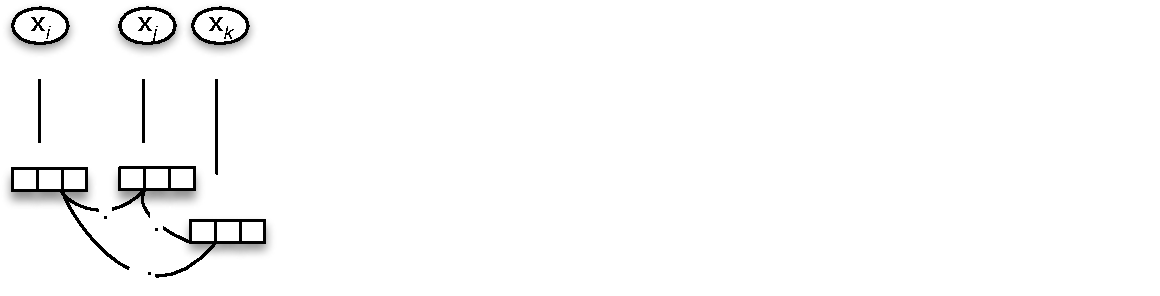
\includegraphics[height=1.75in]{img/diagram_mf.pdf}
%         \caption{\textbf{Shallow}}
%     \end{subfigure}%
%     ~

%     ~
%     \begin{subfigure}[t]{0.22\textwidth}
%         \centering
%         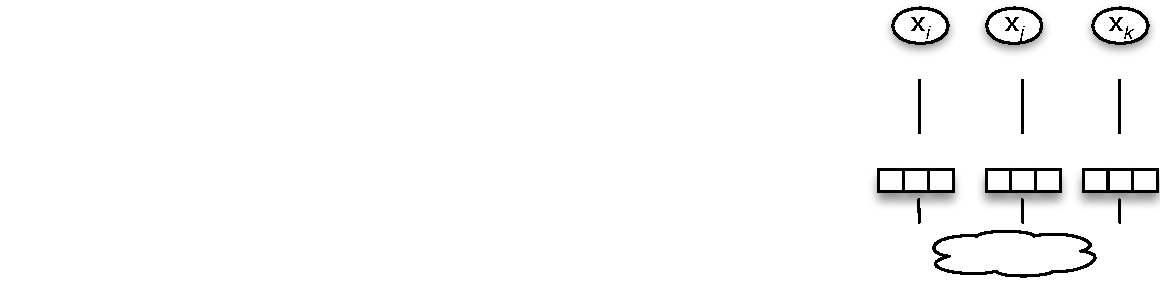
\includegraphics[height=1.75in]{img/diagram_nmf.pdf}
%         \caption{\textbf{``Neural"} \label{fig:neural}}
%     \end{subfigure}
%     \caption{\textbf{Network architectures for factorization models}.  The  white clouds (\Cloud) represent deep layers, for example a convolutional network for text features.
% %    \hl{add label $x_j$ and $x_k$ to figures}
%     \label{fig:architecture}
%     }
% \end{figure*}

% \end{comment}


% More formally, the addition of deep extraction methods yields the following statistical model:


% \begin{align}
% %\hat y(\vect{x}; \vect{b}, \vect{\upphi}, \vect{\upkappa})=
% \omega \biggl(
%                       b_0 +
%                       \sum_{i=1 \vphantom{G(i)}}^n b_i x_i  \; + \;
%                       & \sum_{i =1}^{|\vect{\upkappa}|} \sum_{j=i}^{|\vect{\upkappa}|}   \phi_i( \vect{x}_{\vect{\upkappa}_i}) \dotp \phi_j( \vect{x}_{\vect{\upkappa}_j})
%   \biggr)
%  \label{eq:deepfm}
% \end{align}
% In this notation, $\vect{x}_{\vect{\upkappa}_i}$ is a subvector that contains all of the features that belong to the group $\vect{\upkappa}_i$.
% Thus, $x_{\vect{\upkappa}_i} =  [ x_j : j \in \vect{\upkappa}_i ]$.
% The intuition is that by grouping (sub-)features as a single entity, we can can reason on a higher level of abstraction.
% Instead of individual sub-features interacting among each other, the entities interact with other entities.
% Here, $\phi_i$ is a feature extraction feature that inputs the $i$-th feature group of the instance, and returns an $r$-dimensional embedding.
% The simplest   implementation for $\phi_i$ is a linear fully-connected layer, where the output of the $r$-th entry is:
% \begin{equation}
% \label{eq:fully_connected}
% \phi_i\bigl(\vect{x}_i; \vect{w}\bigr)_r= \sum_{a=1}^{d_i}  w_{r_a} x_{i_a}
% \end{equation}
% The feature extraction function $\phi_i$ can allow for an arbitrary processing of its subfeatures.
% Across groups,  entities interact with  each other via the output of $\phi$ only.
% We can use $\Feat2Vec$ to both use large feature sets and overcome the cold-start problem.
% This is only possible when there is an alternative description of the item available (for example an image or a passage of text).
% In Figure~\ref{fig:cold_start}, we show how we  address this problem by treating the words as indexed features, but placed within a structured feature group $\upkappa_w$.
% A feature extraction function $\phi$ acts on the features in $\upkappa_w$, and the other features interact with the words only via the output of $\phi$.
% Notice that this implies we can precompute and store the latent factors of the labels seen during training, and   predictions  during inference can be sped-up.
% For example if we have two feature groups (e.g, a label and an item),
% first we compute the feature extraction function to the unseen items and their embeddings, and then we simply apply a dot product over the stored vectors of the labels.

% \begin{figure}[htb]
%     \centering
%     \begin{subfigure}[t]{0.25\textwidth}
%         \centering
%         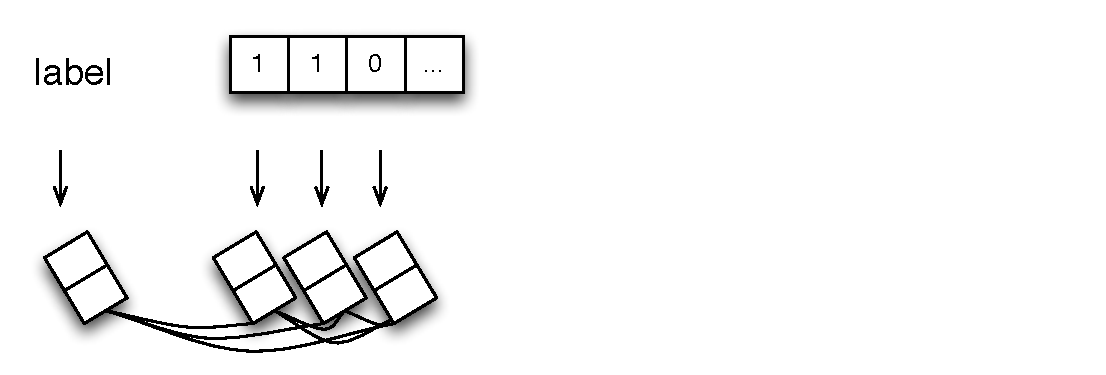
\includegraphics[height=0.75in]{img/cold_start_fm.pdf}
%         \caption{\textbf{Shallow}}
%     \end{subfigure}%
%     ~
%     \begin{subfigure}[t]{0.25\textwidth}
%         \centering
%         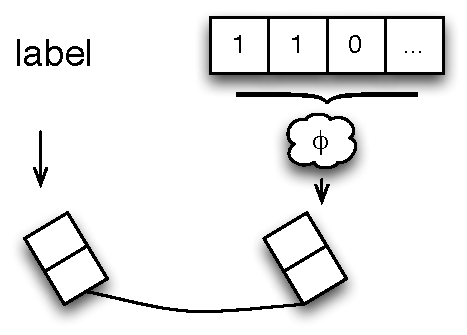
\includegraphics[height=0.75in]{img/cold_start_dsfm.pdf}
%         \caption{\textbf{Deep-In}}
%     \end{subfigure}
%     \caption{  Comparison of how factorization may use item descriptions features.\label{fig:cold_start}
%     }
% \end{figure}




% %Figure~\ref{fig:neural} shows
% Interestingly,  using neural networks within factorization machines  has been proposed multiple times~\cite{DBLP:journals/corr/DziugaiteR15,guo2017deepfm}
% by replacing the dot product of factors with a learned neural function, which has been shown to improve predictive accuracy for various tasks.
% In this case, fast inference for cold-start documents using pre-computed label embeddings is no longer possible.
% However, it would be straightforward to combine this approach with  \algoralph{}, which is not explored in this work.

% $\Feat2Vec$ extends Factorization Machine in two ways:
% it allows grouping of features and it enables arbitrary feature extraction functions.
In this section we describe how $\Feat2Vec$  learns embeddings of feature groups.

\subsection{Model}
\label{sec:algoralph}

%We propose a framework for extending factorization machine with neural methods, by introducing structure into the feature interactions.
%Specifically, we do this by defining  \textit{feature groups},  $\vect{\upkappa}$, where each group contains features of a particular type. Explicitly, $\vect{\upkappa}$ is a partition of the set of feature columns in a dataset and each set within the partition is a feature group.
%For example, the 256 pixel intensities from a $16\times 16$ image may be grouped into an ``image'' feature group.
$\Feat2Vec$ predicts  a target output  $\hat y$ from a list of feature groups constructed from a partition $\vect{\pmb{\upkappa}}$ of raw features ${\vect{\mathbf x}}$:
\begin{align}
  {\vect{\mathbf x}} =   \langle \vect{x}_{\vect \upkappa_1}, \vect{x}_{\vect \upkappa_2}, \dots, \vect{x}_{\vect \upkappa_n} \rangle  = \langle \vect{g}_1, \vect{g}_2, \dots, \vect{g}_n \rangle
 \end{align}
Each of the $n$ feature groups  $\vect{g}_i$ is defined a priori by $\vect \upkappa_i$, which indexes the dimensions in ${\vect{\mathbf x}}$  that belong to the $i$-th group.
For example, we might group together individual words in an item's description into a single ``description text'' feature group. We define an \textit{entity} to be a particular value or realization of a feature group.
The number of dimensions of each group may vary, but all of the feature groups are embedded to the same space via their \textit{feature extraction function} $\phi_i$.
These functions learn how to embed each feature group $\vect{g}_i$ and outputs a vector in $\mathbb{R}^r$.
%In Factorization Machine, all the feature embeddings interact with each other, while in $\Feat2Vec$, the interactions only occur between different feature \textit{groups}.
More, formally:

\begin{align}
%\hat y(\vect{x}; \vect{b}, \vect{\upphi}, \vect{\upkappa})=
\hat y(\vect{\mathbf{x}\vphantom{phi}},\vec{\pmb{\phi}}, \vect{\pmb{\upkappa}\vphantom{phi}} ) = \omega \biggl(
                       \sum_{i =1}^n \sum_{j=i}^n  \overbracket {\phi_i( \vect{x}_{\vect{\upkappa}_i}) }^{ \mathclap  { \text{group $i$}\atop \text{embedding}}} \dotp \overbracket {\phi_j( \vect{x}_{\vect{\upkappa}_j}) }^{ \mathclap  { \text{group $j$}\atop \text{embedding}}}
  \biggr)
 \label{eq:deepfm}
\end{align}

Here $\omega$ is an activation function.
Intuitively, the dot product ($\dotp$) returns a scalar that measures the (dis)similarity between the embeddings of the feature groups.
%$\phi_i$ is a feature extraction that inputs the $i$-th feature group of the instance, and returns an $r$-dimensional embedding.
%The feature extraction function $\phi_i$ can allow for an arbitrary processing of its subfeatures $\vect{x}_{\vect{\upkappa}_i}$.
%Instead of individual sub-features interacting among each other, as in Factorization Machine, the embeddings of feature groups interact with those of other groups.
%Thus, $x_{\vect{\upkappa}_i} =  [ x_j : j \in \vect{\upkappa}_i ]$.
%The intuition is that by grouping features as a single entity, we can can reason on a higher level of abstraction.
%Individual pixels may yield little information about other features in a dataset, such as a review rating, while a single embedding for an entire image may be informative.
%Across groups,  entities interact with  each other via the output of $\phi$ only.
%As a concrete example of an application of this grouping/feature extraction, we might group the individual words of a document into a ``document'' feature group, and allow this document embedding to then interact with learned embeddings of other document metadata (such as author id). We might expect the extraction function $\phi$ for the words in a document to extract features that characterize the attributes of the document taken as a whole, rather than simply the sum of its individual words.
A simple  implementation of $\phi_i$ is a linear fully-connected layer, where the output of the $r$-th entry is:
\begin{equation}
\label{eq:fully_connected}
\phi_{i,r}\bigl( \vect{x\vphantom{\theta}}_i; \vect{\uptheta}_r\bigr )_r= \sum_{a=1}^{d_i}  \theta_{r_a} x_{i_a}
\end{equation}
Other, more sophisticated functional forms of $\phi_i$ we have explored in our experiments include:
\begin{itemize}
\item A convolutional neural network that transforms a text sequence into a $r$-dimensional embedding. This function is able to learn higher order interactions of n-grams, unlike other methods for transforming text to numerical values such as bag-of-words.
\item A deep, fully connected neural network that projects a scalar, such as average rating, into a $r$-dimensional embedding space. This extraction function, by treating the input as numerical, will require scalars close in value to have similar embeddings.
\end{itemize}
Any neural function that outputs a $r$-dimensional vector could be plugged into our framework as an extraction function $\phi$.



% As a concrete example of feature grouping, consider a user-level dataset with information on past purchases of 2 products ($p_1,p_2$) and 2 shipping locations ($l_1,l_2$). A data scientist may want interactions to occur exclusively between locations and purchases, because they believe interactions between purchases or between locations are non-informative. There would then be 2 feature groups: all recorded purchases, and all recorded shipping locations:
% $\vect{\upkappa} = \{ \{p_1,p_2 \}, \{ l_1 , l_2 \}  \}$
%Note that without loss of generality, we could define a model that is equivalent to a Factorization Machine by requiring each feature group to be a singleton :
%$
%\vect{\upkappa} = \{ \{x_1\}, \{ x_2 \}\ldots \{ x_n \} \}
%$ and the linear extraction function presented in Equation \ref{eq:fully_connected}.


Figure~\ref{fig:architecture} compares existing factorization methods  with our novel model in diagram form.
%To graphically demonstrate the difference between Factorization Machine and
Figure~\ref{fig:factorization_machine} shows a Factorization Machine~\cite{rendle2010factorization} that embeds each feature .
In this example, Figure~\ref{fig:feat2vec}  shows $\Feat2Vec$ with two feature groups:
the first group only has a single feature which is projected to an embedding (just like matrix factorization);
but the second group has multiple features, which are together projected to a single embedding.
%Consider how we can use $\Feat2Vec$ to overcome the cold-start problem.
Figure~\ref{fig:neural} shows an approach of using neural networks within factorization machines  that has been proposed multiple times~\cite{DBLP:journals/corr/DziugaiteR15,guo2017deepfm}.
It replaces the dot product of factors with a learned neural function, which has been shown to improve predictive accuracy.
The caveat of this architecture is that is no longer  possible to interpret the embeddings as latent factors related to the target task.

In traditional factorization methods, individual item identifiers are embedded and thus need to be observed during training (i.e., cold-start problem).
 $\Feat2Vec$ can learn an embedding from an alternative characterization of the item---for example, an item's textual description.
For this, we  can treat the entire textual description as a feature group $\upkappa_i$. %the group of word features.
A feature extraction function $\phi_i$ acts on the features in $\upkappa_i$, and the other features interact with the words only via the output of $\phi_i$.
%However, $\Feat2Vec$ is not limited to bag of words features, and we  demonstrate this with continuous features.


%Notice that this implies we can precompute and store the latent factors of the target task seen during training, so that predictions  during inference can be sped-up.
%For example if we have two feature groups (e.g, a label and an item),
%first we compute the feature extraction function to the unseen items and their embeddings, and then we simply apply a dot product over the stored vectors of the labels.

%\begin{figure}[htb]
%    \centering
%    \begin{subfigure}[t]{0.25\textwidth}
%        \centering
%        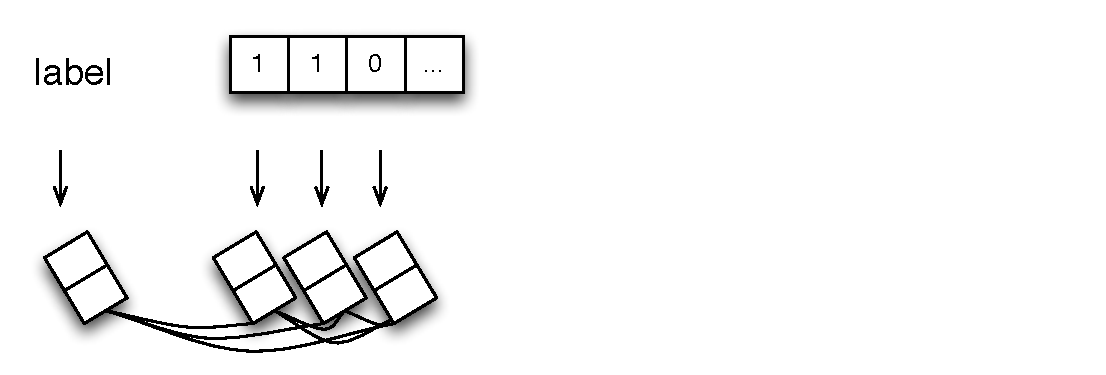
\includegraphics[height=0.75in]{img/cold_start_fm.pdf}
%        \caption{\textbf{Shallow}}
%    \end{subfigure}%
%    ~
%    \begin{subfigure}[t]{0.25\textwidth}
%        \centering
%        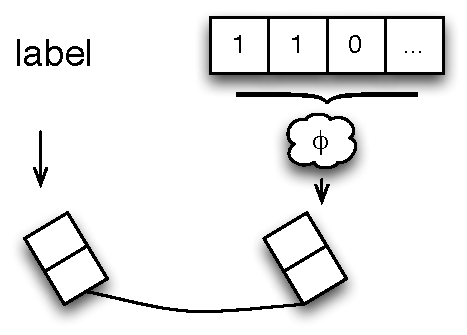
\includegraphics[height=0.75in]{img/cold_start_dsfm.pdf}
%        \caption{\textbf{Feat2Vec}}
%    \end{subfigure}
%    \caption{  Comparison of how factorization may use item descriptions features.\label{fig:cold_start}
%    }
%\end{figure}


% \begin{align}
% \lambda^{\text{s}}(\vect{x}, \vect{w}, \vect{I}, \vect{J} ) \triangleq &
% \end{align}
% For example, consider a model with four features ($n=4$).
% In a shallow model, a feature interacts with all other features,



\begin{figure*}[th]
    \centering
    \begin{subfigure}[t]{0.26\textwidth}
        \centering
        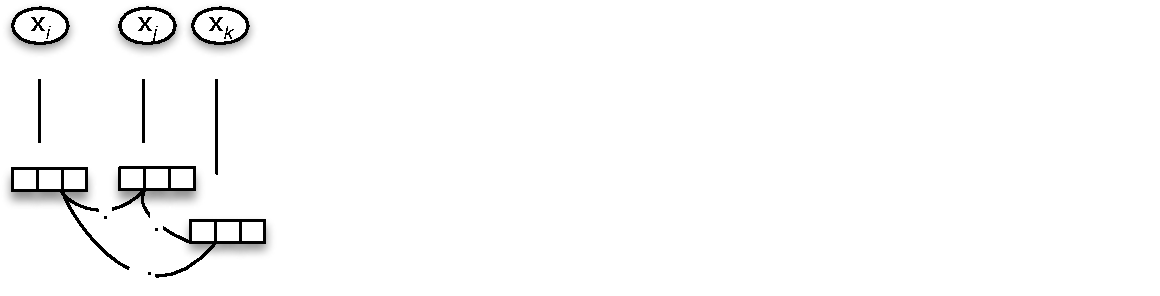
\includegraphics[height=1in]{img/diagram_mf.pdf}
        \caption{\textbf{Factorization Machine}\label{fig:factorization_machine}}
    \end{subfigure}%
    ~
    \begin{subfigure}[t]{0.26\textwidth}
        \centering
        
\includegraphics[height=1in]{img/diagram_in.pdf}
        \caption{\textbf{Feat2Vec} \label{fig:feat2vec}}
    \end{subfigure}
    ~
    \begin{subfigure}[t]{0.22\textwidth}
        \centering
        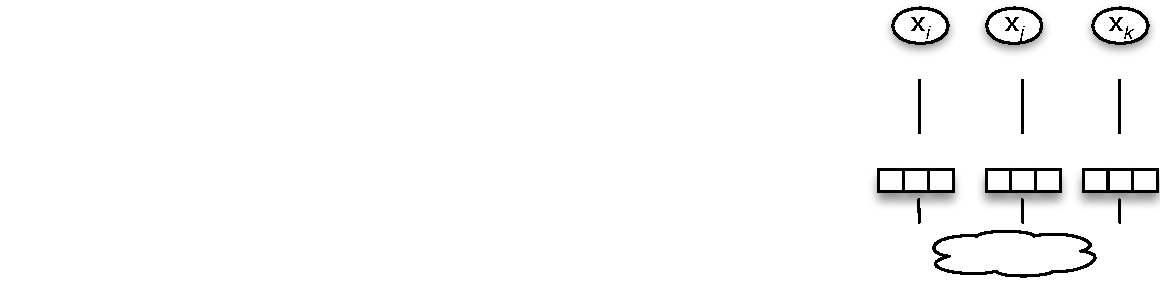
\includegraphics[height=1in]{img/diagram_nmf.pdf}
        \caption{\textbf{``Neural"} \label{fig:neural}}
    \end{subfigure}
    \caption{\textbf{Network architectures for factorization models}.  The  white clouds (\Cloud) represent deep layers, for example a convolutional network for text features, while the dots ($\cdot$) denote dot products.
%    \hl{add label $x_j$ and $x_k$ to figures}
    \label{fig:architecture}
    }
\end{figure*}


The structure of the $\Feat2Vec$ model significantly expands previously published models.
For example, Principal Component Analysis (PCA) is a common method to learn embeddings of individual dimensions of  data.
Although structured regularization techniques exist~\cite{jenatton2010structured}, it is not obvious how to combine different dimensions in PCA when we are interested in treating a subset of dimensions as a single group, such as words in an item's description.
%For example, consider a dataset that has a textual description of items--- we may be interested in having an embedding for the feature group (the entire description) instead of the individual words.
$\Feat2Vec$ extends Factorization Machine~\cite{rendle2010factorization}, in that we allow calculating embeddings for feature groups and we use feature extraction functions.
StarSpace~\cite{wu2017starspace}  introduces feature groups (called entities in their paper), but is only compatible with supervised tasks, constrains  groups to be ``bags of features'', and is limited to two feature types.
In contrast, $\Feat2Vec$ allows any number of groups to enter the model, and is compatible with diverse types of data, such as continuous features or ordered sequences.

Additionally, we introduce a new implicit sampling method that enables learning self-supervised embeddings for feature groups.
% replaced n <- p;  because we use p for probabilities
Unlike $\Word2Vec$, a popular self-supervised embedding algorithm, we do not constraint features types to be words.
%Features groups can be  individual columns in a data matrix,  but they need not to be.
Instead, by grouping features using the hyperparameter $\vect{\pmb{\upkappa}}$ in Equation \ref{eq:deepfm}, the self-supervised model can reason on more abstract entities in the data.
For example, in our experiments on a movie dataset, we are able to define a ``genre'' feature group, where we group non-mutually exclusive indicators for movie genres, including comedy, action, and drama films. This embedding may capture complex interactions between genre classifications typically unavailable through a tokenized treatment of genres.



%However, it would be straightforward to combine this approach with  \algoralph{}. This is not explored in this work.



\subsection{Supervised Learning from Data}
\label{sec:learning_supervised}

We can learn the the parameters of a Feat2Vec model $ \bm\uptheta$ using training data by minimizing a loss function $\mathcal L$:
\label{sec:learning}
\begin{equation}
\arg \min_{\vect{\uptheta}} \sum_x  \mathcal{L}\bigl(  y(x), \hat y(x;\vect{\uptheta})\bigr) + \gamma ||  \bm{\uptheta}||_{2}
\label{eq:learning}
\end{equation}
Here, $y(x)$  is the true target value for $x$ obtained from training data, and $\hat{y}(x)$ is the one estimated by the model (Equation \ref{eq:deepfm});
$\bm\uptheta$ represents the parameters learned in during training (i.e. the parameters associated with the extraction functions $\phi_i$).
The hyperparameter $\gamma$ controls the amount of regularization.
For labeling and classification tasks, we optimize the binary cross-entropy.

%for $y \in \{0, 1\}$:
%\begin{equation}
%\mathcal{L}(y, \hat{y}) =  -\bigl(y\, \log(\hat y)\bigr)  - (1- y) \log(1- \hat{y}) \bigl)
%%  -(yt log(yp) + (1 - yt) log(1 - yp))
%\label{eq:crossentropy}
%\end{equation}
%For the regression tasks where the target value is continuous, we optimize the mean squared error (MSE):
%\begin{equation}
%\mathcal{L}(y, \hat{y}) = (y-\hat{y})^2
%\label{eq:mse}
%\end{equation}

%Neural models  are typically learned using mini-batch updates, where the incremental descent is performed with respect to several instances at a time.
%For the implementation of this paper, we built our models using the Keras programming toolkit~\cite{chollet2015keras}, that is now part of Tensorflow~\cite{tensorflow2015-whitepaper}.
%It enables automatic differentiation, and is bundled with
% a general-purpose optimization algorithm called ADAM~\cite{kingma2014adam} that needs no tuning of  gradient  step sizes.

It is straightforward to optimize Equation~\ref{eq:learning} directly.
Typically, this loss will be for a prediction task, and involve at least two feature groups---one of the feature groups is the target label that we want to predict, such as rating, and the other group(s) is the input from which we want to make the prediction, such as review text.

Consider a target feature group $g_i$ that exists in a high dimensional space.
This could be a one-hot encoding of a categorical variable with a large number of possible values.
In such a scenario, it may be too costly to feed the model all negative labels, particularly if the model is sparse.
In these cases, we can instead use a binary classifier with implicit sampling~\cite{samplingnotes}, where we  sample a fixed number ($k$) from the set of possible negative labels for each positively labeled record.
%In implicit sampling, instead of using all of the possible negative labels, one simply samples a fixed number ($k$) from the set of possible negative labels for each positively labeled record.
This makes our Feat2Vec model feasible to implement for high-dimensional target features.
%$\Word2Vec$ makes use of an algorithm called Negative Sampling, that has little theoretical guarantees~\cite{samplingnotes}.
%For the multi-label classification tasks, we use $\Feat2Vec$ with a binary output.

%The output indicates whether the label is associated in the data with the input ($y=1$), or not ($y=0$).
%The datasets we use for our labeling experiments only contains positive labels, thus for each training example we sample $k$ negative labels for each positive label.
%It is typical to use one of the following negative sampling strategies according to the best validation error, in each case excluding the actual positive labels for each training example -- (i) uniformly from all possible labels, or (ii)  from the empirical distributions of positive labels~\cite{improving_pairwise_learning}.
%EXCLUDED bayesian_pairwise_ranking,; duplicitous reference.


\subsection{Self-supervised Learning From Data}
\label{sec:sampling}

We now discuss how $\Feat2Vec$ can be used to learn embeddings in an self-supervised setting with no explicit target for prediction.
%\subsubsection{Sampling for Unsupervised Learning}

%For more involved feature types (e.g., an image),  one would need to  define a function $\phi$ that builds intermediate layers  to map the entity to an embedding .


The training dataset for a $\Feat2Vec$ model consists of the observed data.
In natural language, these would be documents written by humans, along with document metadata.
Since self-supervised Feat2Vec will require positive and negative examples during training, we supply unobserved data as negative examples.
This is analogous to $\Word2Vec$, which samples a negative instance from a noise distribution $\q_{w2v}$ that is proportional to the empirical frequency of a word in the training data.


We start with a dataset $S^+ $ of records with $n$ feature groups.
We then mark all observed records in the training set as our positive-labeled examples.
For each positive record, we generate $k$ negative labels using the 2-step algorithm documented in Algorithm \ref{algo:samp}:

\begin{algorithm}[htb]
 \caption{Implicit sampling algorithm for self-supervised $\Feat2Vec$}
 \label{algo:samp}
\begin{algorithmic}[1]
\footnotesize
\Function{Feat2Vec\_Sample}{$S^+, k, \alpha_1, \alpha_2$}
\State $S^-  \leftarrow \emptyset $
\For {$\vect{x}^{\,+} \in S^+ $}
	\State Draw a random feature group $\upkappa_i  \sim \q_1(\{\operatorname{params}(\phi_i)\}_{i=1}^{|\vect{\upkappa}|},\alpha_1) $
	\For {$j \in \{1,\ldots,k\}$}
			\State $\vect{x}^{\,-}  \leftarrow \vect{x}^{\,+} $ \Comment  set initially to be equal to the \begin{flushright}positive sample\end{flushright}
			\State Draw a random entity  $\tilde x \sim \q_2(\mathrm{X}_{ \upkappa_i },\alpha_2)$
			\State $\vect{x}^{\,-}_{\upkappa_i}  \leftarrow \tilde x$ \Comment{substitute the $i$-th feature group \begin{flushright}with the sampled one\end{flushright}}
			\State  $S^-  \leftarrow S^-  + \{  \vect{x}^{\,-} \}$
	\EndFor
\EndFor
\State \Return $S^-$
\EndFunction
\end{algorithmic}
\end{algorithm}


Explained in words, our negative sampling method for self-supervised learning iterates over all of the observations of the training dataset.
For each observation $\vect{x}^{\,+}$, it randomly selects the $i$-th feature group from a noise distribution $\q_1(\cdot)$.
Then,  it creates a negative observation that is identical to $\vect{x}^{\,+}$, except that its $i$-th entity is replaced by a value sampled from a noise distribution $\q_2(\cdot)$.
In our application, we use the same class of noise distributions (flattened multinomial) for both levels of sampling, but this need not be the case.
We now describe the noise distributions that we use.
Let  $P_{\q}(x)$ denote the probability of $x$ under distribution $\q$.

\textbf{Sampling Feature Groups.}
To sample a feature group, we choose a feature group $\upkappa_i$ from a multinomial distribution with probabilities proportional a feature's complexity.
By complexity, we mean the number of parameters we learn that are associated with a feature group's extraction function $\phi_i$.
This noise distribution places more weight on features that have more parameters and thus are going to require more training iterations to properly learn. The sampling probabilities of each feature group are:

\begin{equation}
P_{\q_1}(\upkappa_i|\operatorname{params}(\phi_i)\}_{i=1}^{|\vect{\upkappa}|},\alpha_1 )  \
= \frac{\operatorname{params}(\phi_i)^{\alpha_1}}{\sum_{j=1}^{|\vect{\upkappa}|} \operatorname{params}(\phi_j)^{\alpha_1}}
\end{equation}
where the function $\operatorname{params}$ calculates the complexity of a  feature extraction function $\phi_i$.
For categorical variables using a linear fully-connected layer, the complexity is simply proportional to the number of categories in the feature group.
However, if we have multiple intermediate layers for some feature extraction functions (e.g., convolutional layers), these parameters should also be counted towards a feature group's complexity.
The hyper-parameter $\alpha_1 \in [0,1]$ flattens the distribution.
 When  $\alpha_1=0$, the feature groups are sampled uniformly,
 and when $\alpha_1=1$, they are sampled exactly proportional to their complexity.
%Figure \ref{fig:alpha} in the Appendix provides a visualization of how the feature sampling rate varies with the hyperparameter for features with differing levels of complexity.


\textbf{Sampling Entities.}
To sample an entity within a feature group $\upkappa_i$, we use a similar strategy to $\Word2Vec$ and sample from the empirical distribution of values:
%For  $\q_2(\mathrm{X}_{\upkappa_i}, \alpha_2)$, is the ``flattened'' empirical multionomial distribution over the frequency of the feature values of feature $\upkappa_i$, as in the negative sampling procedure used in $\Word2Vec$ :
\begin{equation}
P_{\q_2}(x|\mathrm{X}_{\upkappa_i},\alpha_2)  \
= \frac{ \operatorname{count}(x)^{\alpha_2}}{\sum_{x_{\upkappa_i}' \in S^+ } \operatorname{count}(x_{\upkappa_i}')^{\alpha_2}}, \quad \alpha_2 \in [0,1]
\end{equation}
Here, $\operatorname{count}(x)$ is the number of times a value $x$ of feature group $i$ appeared in the training dataset $S^+$ , and $\alpha_2$ is again a flattening hyperparameter.


This method will sometimes by chance generate negatively labeled samples that \textit{do} exist in our sample of observed records.
The literature offers two solutions:
in the Negative Sampling of $\Word2Vec$, duplicate negative samples are ignored~\cite{samplingnotes}.
Instead, we account for the probability of random negative labels being identical to positively labeled data using \textit{Noise Contrastive Estimation} (NCE)~\cite{nce}.

%%%%%%%%%%%%%%%%
\subsubsection{The Loss Function for Self-Supervised Learning}
\label{sec:learning}
For our self-supervised learning of embeddings, we optimize a NCE loss function, to adjust the structural statistical model
$\hat y = p(y=1|\vect{x},\vect{\phi}, \bm\uptheta)$
expressed in Equation \ref{eq:deepfm}, to account for the possibility of random negative labels that appear identical to positively labeled data.
Since in self-supervised learning we only deal with a dichotomous label, indicating a positive or negative sample, we restrict our attention to usage of Equation \ref{eq:deepfm} with $\omega$ as a logistic link function.

An additional burden of NCE is that we need to calculate a partition function $Z_{\vec{x}}$ for each unique record type $\vec{x}$ in the data that transforms the probability $\hat y$ of a positive or negative label into a well-behaved distribution that integrates to 1.
This would introduce an astronomical amount of computation and greatly increase the complexity of our model.
Instead, we appeal to the work of \citet{fastnnlang},
who show that in the context of language models setting the $Z_{\vec{x}}=1$ in advance does not change the performance of the model.
The intuition is that if the underlying model has enough free parameters, it will effectively learn the probabilities itself, since systemic under/over prediction of probabilities will result in penalties on the loss function.
%change notation to be in terms of phi and w the weights
Written explicitly, the new structural probability model is:
\begin{equation}
\tilde p(y=1|\vec{x\vphantom{phi}},\vec{\phi}, \bm\uptheta) = \frac{\exp\bigl(s(\vec{x\vphantom{phi}}|\vec{\phi}, \bm\uptheta) \bigr)}{\exp( s\bigl(\vec{x\vphantom{phi}}|\vec{\phi}, \bm\uptheta), \bigr) + P_{\q}(\vec{\vphantom{phi}x}| \alpha_1,\alpha_2)}
\end{equation}
%where:
\begin{equation}
s(\vec{x\vphantom{phi}}|\vec{\phi}, \bm\uptheta) =
                       \sum_{i =1}^{|\vect{\upkappa}|} \sum_{j=i}^{|\vect{\upkappa}|}   \phi_i( \vect{x}_{\vect{\upkappa}_i}) \dotp \phi_j( \vect{x}_{\vect{\upkappa}_j})
\end{equation}
$s(.)$ denotes the score of a record $\vec{x}$ given parameters/extraction functions,
and $P_{\q}(.)$ denotes the probability of a record $\vec{x}$ being drawn from our negative sampling algorithm, conditional on the positively labeled record $\vect{x}^+$ the negative sample is drawn for:
\begin{align*}
P_{\q}(\vec{x}|\alpha_1,\alpha_2,\mathrm{X},\vect{x}^+) = P_{\q_2}(\vec{x}_{\upkappa_i}|\mathrm{X}_{\upkappa_i},\upkappa_i,\alpha_2)\times \\ P_{\q_1}(\upkappa_i|\operatorname{params}(\phi_i)\}_{i=1}^n,\alpha_1)
%\text{\hl{Write equation!! This is only defined in the middle of the appendix}}
\end{align*}

Our loss function $L$ optimizes $\bm\uptheta$, the parameters of the feature extraction functions $\vect\phi$, while accounting for the probability of negative samples.
\begin{align*}
L(S) & = \arg\min_{\bm\uptheta}   \frac{1}{|S^+|} \sum_{\vect{x}^{\,+} \in S^+} \Big(\log(\tilde p(y=1|\vect{x}^{\,+},\vec{\phi},\bm\uptheta   ) ) \; + \\
&  \sum_{\vect{x}^{\,-}  \sim \q(\cdot|\vect{x}^+)}^k \log(\tilde p(y=0|\vect{x}^{\,-},\vec{\phi},\bm\uptheta   )) \Big)
\end{align*}


$\Feat2Vec$ has interesting theoretical properties.
% It is well known that Factorization Machines can be used as a multi-label classifier:
% with at least two features, one can use one feature as a target label, and the other(s) as the input feature to make a prediction.
% In such setting, the output indicates whether the label is associated with the input ($y=+1$), or not ($y=0$), and therefore the input can be associated with more than one label.
With $n$ feature groups, the loss function of self-supervised $\Feat2Vec$ can be shown to be equivalent to  a convex combination of the losses from $n$ supervised $\Feat2Vec$ models with implicit sampling (proof omitted).
In other words, it optimizes $n$ multi-label classifiers, where each classifier  is optimized for a different target feature group. Intuitively, during sampling in self-supervised Feat2Vec, we choose a random target feature group according to $P_{\q_1}$, and then add that specific group's supervised loss to the total self-supervised loss.


\section{Empirical Results}
\label{sec:evaluation}

\subsection{Supervised Embeddings}
\label{sec:targeted embeddings}

We now address our working hypotheses for evaluating supervised embeddings.
We evaluate  on the Yelp dataset\footnote{https://www.yelp.com/dataset/challenge}, which consists of 4.7 million reviews of restaurants.
%To avoid overfitting, for all our experiments we define a training, development and a test.
For all of our experiments, we define a development set and a single test set which is 10\% of the dataset, and a part of the development set is used for early stopping or validating hyper-parameters.
%Since these datasets are large and require significant time to train on an Nvidia K80 GPU cluster, we report results on only a single training-test split.
%For the multi-label classification task in \ref{sec:coldstart} we predict a probability for each document-label pair and use an evaluation metric called Area Under the Curve (AUC) of the Receiver Operating Characteristic (ROC).
%A caveat of our evaluation strategy is that we could be underestimating the performance of our models---there is a small probability that  the sampled negatives labels are false negatives.
%However, since we apply the same evaluation strategy consistently across our methods and baselines, the relative difference of the AUC is meaningful.
%We choose the AUC as a metric because it is popular for both classification and ranking problems.
We use mean squared error (MSE) as the evaluation metric for predicting ratings in the Yelp dataset.
%In preliminary experiments we noticed that regularization slows down convergence with no gains in prediction accuracy, so we avoid overfitting only by using early stopping.
We share most of the code for the experiments online\footnote{\url{https://goo.gl/zEQBiA}}.

% Table~\ref{deepout-datasetsl} provides descriptive statistics of the datasets that we consider.
We build 3 feature groups for this task: item (restaurant) identifiers, user identifiers, and review text.
We use a standard linear (Equation \ref{eq:fully_connected}) extraction functions $\phi$  on each one-hot encoding representation of users and items.
For our feature extraction function for review text, we use  a Convolutional Neural Network (CNN), which  has been shown to be effective for natural language tasks~\cite{DBLP:journals/corr/KalchbrennerGB14,tagspace}.
%In Appendix~\ref{appendix:cnndetails} we describe this network  and its hyper-parameters.
Instead of tuning the hyper-parameters, we follow previously published  guidelines~\cite{zhang2015sensitivity}.

% \begin{table}[]
% \footnotesize
% \centering
% \caption{Details of labelling task datasets}
% \label{deepout-datasetsl}
% \begin{tabular}{@{}llllll@{}}
% \toprule
%                 & \begin{tabular}[c]{@{}l@{}}Number of \\ documents\end{tabular} & \begin{tabular}[c]{@{}l@{}}Total number \\ of labels\end{tabular} & \begin{tabular}[c]{@{}l@{}}Mean labels \\ per document\end{tabular} & \begin{tabular}[c]{@{}l@{}}Mean document \\ length (words)\end{tabular} & \begin{tabular}[c]{@{}l@{}}Negative label\\ sampling strategy\end{tabular} \\ \midrule
% Concepts        & 42,710                                                         & 186,215                                                           & 117                                                                 & 2,117                                                                   & Uniform                                                                    \\
% Skills          & 544,388                                                        & 25,299                                                            & 72                                                                  & 276                                                                     & Empirical                                                                  \\
% CiteULike users & 16,980                                                         & 5,551                                                             &    12                                                                &                        195                                                & Empirical                                                                  \\ \bottomrule
% \end{tabular}
% \end{table}


\begin{comment}
\subsubsection{ Is \algoralphabbr{} effective for cold-start predictions? }
\label{sec:coldstart}
We compare $\Feat2Vec$ with an extension of matrix factorization that can generalize to unseen items for text documents, Collaborative Topic Regression (CTR-- \citet{wang2011collaborative}), a method with an  open-source Python implementation\footnote{https://github.com/arongdari/python-topic-model}.
We evaluate them on the  \textbf{CiteULike}  dataset which consists of pairs of scientific articles and the users who have added them to their personal libraries, and it contains 16,980 unique articles and 5,551 unique users.
We use the models to predict users who may have added a given article to their library.
We compare the performance of \algoralph{} with CTR using pre-defined cross-validation splits\footnote{For warm-start we use
\url{https://www.cs.cmu.edu/~chongw/data/citeulike/folds/cf-train-1-items.dat} and for cold-start predictions, we use the file \texttt{ofm-train-1-items.dat} and the corresponding test sets for each}.
 We use 1\% of the training set for early stopping.


For CTR we use the hyper-parameters reported by the authors as best, except for $r$ which we found had a significant impact on training time .
We only consider $r \in \{5,10,15\}$ and choose the value which gives the best performance for CTR.
On the warm-start condition,  CTR has an AUC of 0.94;
however, it shows significant degradation in performance for unseen documents and it only performs at random chance with an AUC of 0.50.
On the other hand, \algoralphabbr{} achieves AUC of 0.94 on the warm-start condition, and it only degrades to 0.91 on unseen documents.
\algoralphabbr{} can also be trained over ten times faster, since it can leverage GPUs.\footnote{\algoralphabbr{} and MF were trained on an Nvidia K80 GPU, while CTR was trained on a Xeon E5-2666 v3 CPU.}
We also note that we have not tuned the architecture or hyper-parameters of the feature extraction function $\phi$ and greater improvements are possible by optimizing them.



% \begin{table}
% \footnotesize
% \begin{centering}
% \setlength\tabcolsep{4pt}
% \begin{minipage}{0.55\textwidth}


% \caption{Labeling results for warm-start documents}
% \label{tbl:inmatrixresults}
% \begin{tabular}{@{}lllll@{}}
% \toprule
%                      & \multicolumn{2}{c}{Concepts}  & \multicolumn{2}{c}{Skills}     \\
% Model                & AUC  & Train mins. & AUC  & Train mins. \\ \midrule
% $\Feat2Vec$            & \textbf{0.92} & 1,876                  & \textbf{0.65} & 3,256                   \\
% Matrix Fact. & 0.88 & \textbf{64}                     & 0.61 &  \textbf{8}                      \\
% \end{tabular}

% \end{minipage}
% \hfill
% \begin{minipage}{0.4\textwidth}



% \end{minipage}
% \end{centering}

% \end{table}




% \begin{tabular}{@{}lll@{}}
% \label{ratingpredtable}
% \caption{Yelp rating prediction}

% \toprule
%                      & MSE    & \begin{tabular}[c]{@{}l@{}}Improvement over MF\end{tabular} \\ \midrule
% Matrix Factorization & 1.561 & -                                                                                         \\
% $\Feat2Vec$  &   \textbf{0.480}     & \textbf{69.2} \%                                                                                  \\
% DeepCoNN             &  1.441    & 19.6 \%
% \end{tabular}
\end{comment}


\begin{table}[]
\centering
\caption{Supervised Yelp rating prediction}
\label{ratingpredtable}
\begin{tabular}{@{}lcc@{}}
\toprule
                     & MSE   & Improvement over MF \\ \midrule
Feat2Vec             & \textbf{0.480} &  \textbf{69.2} \%                                 \\
DeepCoNN             & 1.441 & 19.6 \%                                \\
MF (Matrix   & 1.561 & -                                      \\
Factorization) \\
\bottomrule
\end{tabular}
\end{table}


\subsubsection{Comparison with alternative CNN-based text factorization}
\label{ratingpred}
We now compare  with a method called DeepCoNN, a deep network specifically designed for  incorporating text into matrix factorization~\cite{deepconn}, a state of the art method for predicting customer ratings when text reviews are available.
To make results comparable, the \algoralphabbr{} experiments use the same feature extraction function used by DeepCoNN.
For each user-item pair, DeepCoNN concatenates the text from all reviews for that item and all reviews by that user.
The concatenated text is then fed into a feature extraction function for each entity, followed by a factorization machine.


Table \ref{ratingpredtable} compares our methods to  DeepCoNN's published results  because a public implementation is not available.
\algoralph{} provides a large performance increase when comparing the  reported improvement in the mean squared error (MSE) over Matrix Factorization,
Our approach is more general, and we claim that it is also  more efficient.
Since DeepCoNN concatenates text, when the average reviews per user is $\bar{n_u}$  and reviews per item is $\bar{n_i}$, each text is duplicated on average $\bar{n_i}\times \bar{n_u}$ times per training epoch.
In contrast, for \algoralphabbr{} each review is seen only once per epoch.
Thus it can be 1-2 orders of magnitude more efficient for datasets where $\bar{n_i}\times \bar{n_u}$ is large.


\subsection{Self-Supervised Embeddings}
\label{sec:unsupexp}
%\subsubsection{Does $\Feat2Vec$ enable better embeddings?}
The prediction of similar or related words is a commonly used method for evaluating self-supervised word embeddings~\cite{bojanowski2016enriching,mikolov2013efficient}.
Since our algorithm is designed for multi-modal data, we generalize this task for multiple feature types as follows.
Given a dataset with $n$ feature groups $g_1,g_2,\ldots g_n$ we have trained a self-supervised $\Feat2Vec$ model on, we choose one group $g_i$ as the ``target'' and a group $g_j$ as the predictor.
Given a held-out instance, we rank all possible values of the target group by cosine similarity to the predictor group's embedding $\phi_j( \vect{x}_{\vect{\upkappa}_j})$ for that instance. We then retrieve the ranking of the actual target entity for the held-out instance in the test dataset.
Rankings are evaluated according to  their  mean percentile rank (MPR):
$MPR = \frac{1}{N}\sum_{i=1}^N R_i/(\max R)$, where $R_i$ is the the target entity rank for instance $i$.
A score of 0 would indicate perfect performance (i.e. top rank every test sample given), so a lower value is better under this metric.
We will use this method to compare the performance of $\Feat2Vec$ algorithm and compare its performance to $\Word2Vec$'s CBOW algorithm for learning embeddings. In our experiments, we set $\alpha_1=.25$, $\alpha_2=0.75$, $k=5$ and $r=50$. We evaluate self-supervised $\Feat2Vec$  on 3 datasets:
%In particular, in the movie dataset we  compare the similarity of movie directors to those of actors who were cast in the same film for a left-out set of films.
%For our educational dataset, we compare rankings of textbooks by evaluating the similarity of textbook and user embeddings.
 %See the appendix \S\ref{sec:imdbexp} for further details on the experimental setup.

%\item The next is mean reciprocal rank (MRR), which is similar to mean percentile rank, but weights rankings that are closer to rank 0 (the best rank possible) more:
%\begin{align*}
%MRR = \frac{1}{N}\sum_{i=1}^N \frac{1}{R_i+1}
%\end{align*}
%The idea behind this metric is that, under MPR, an improvement  in rankings under an algorithm from  10 to 1 will be equally weighted as an improvement from 49,103 to 49,92 in terms of calculating the $MPR$ statistic.
%Clearly, the former improvement is more useful in a real-world context of submitting reccomendations to users, and so MRR attempts to correct for this by weighting rankings closer to 1 much higher.
%A higher value, unlike MPR, indicates better performance.
%\item The final metric we consider is top 1 precision, or the percent of test examples we successfully rank the entity as the top prediction.
%\end{itemize}

%
% \subsubsection{Datasets}

\paragraph{Movies}
The Internet Movie Database (IMDB) is a publicly available dataset\footnote{\href{http://www.imdb.com/interfaces/}{http://www.imdb.com/interfaces/}} of information related to films, television programs and video games.
We limit our experiments to data on its 465,136 movies.
%Table~\ref{tab:features} in the appendix (\S\ref{sec:imdbexp}) summarizes the feature types we use.
Table \ref{tab:features} summarizes our feature groups. For categorical features within a group, we learn a unique embedding for each value.
For groups with multiple categories, we use a ``Bag of categories'' approach to produce a group embedding.
For example, we sum learned embeddings of individual actors such as Tom Cruise to produce a single ``actor'' feature group embedding associated with a title. For real-valued features, we pass the scalar output through a fully-connected 3-layer neural network to output an $r$-dimensional embedding.


\paragraph{Education}
%We use a dataset from \hl{Anonymized}, a leading technology company that provides educational services.
We use a dataset from an anonymized leading technology company that provides educational services.
In this proprietary dataset, we have 57  million observations and 9 categorical feature types which include textbook identifier, user identifier, school identifier,
%and course the book is typically used with,
along with other proprietary features.
Each observation is an interaction a user had with a textbook.

\paragraph{Yelp}
We use the Yelp dataset from our supervised experiments to evaluate the efficacy of self-supervised embeddings in ratings prediction.
%, compared to traditional self-supervised word embedding algorithms Doc2Vec and Word2Vec (CBOW).

\begin{table}[htb]
\footnotesize
\caption{IMDB Feature Groups}
\label{tab:features}
\begin{tabular}{@{}lllp{6cm}@{}}
\toprule
% Created with: https://www.tablesgenerator.com/
Feature Group      & Type              & \# of feats.  \\ \midrule
Runtime (minutes)       & Real-valued       & 1          \\
IMDB rating (0-10)      & Real-valued       & 1          \\
\# of rating votes & Real-valued       & 1           \\
Is adult film?          & Categorical           & 2         \\
Movie release year      & Categorical          & 271      \\
Movie title             & Bag of Words      & 165,471       \\
Directors               & Bag of categories & 174,382                          \\
Genres                  & Bag of categories & 28                  \\
Writers                 & Bag of categories & 244,241             \\
Principal actors & Bag of categories & 1,104,280      \\\bottomrule
\end{tabular}
\end{table}



\subsubsection{Results}

After training IMDB embeddings, we use cast members associated with movies in the test set and predict the actual director of the film.
%If there is a cast member in the test dataset who did not appear in the training data, we exclude them from the summation.
For the educational dataset, we directly  retrieve the most similar textbooks to the user embedding.

Table \ref{tab:eval} presents our evaluation results.
$\Feat2Vec$ outperforms CBOW in the MPR metric.
Additionally, while CBOW predicts the actual director 1.26\% of the times, $\Feat2Vec$ does so 2.43\% of the time, a 92\% improvement in Top-1 Precision over CBOW.
%We explore in greater detail the distribution of the rankings in the appendix in \S\ref{sec:imdbdist}.



\begin{table}[htb]
\footnotesize
\centering
\caption{Mean percentile rank}
\begin{tabular}{lcc}
\hline
Dataset & $\Feat2Vec$ & CBOW \\ \hline
IMDB & 19.36\% & 24.15\% \\
Educational & 25.2\% & 29.2\% \\
\hline
\end{tabular}
\label{tab:eval}
\end{table}



\subsection{Self-Supervised $\Feat2Vec$ Performance with Continuous Inputs}
%^We can probably wordsmith this
%One of our goals in this work is a general-purpose algorithm that can handle arbitrary features.
%We study  $\Feat2Vec$'s performance on a continuous feature. %non-categorical features, we evaluate the embeddings calculated using
We now focus on how well $\Feat2Vec$ performs on a real-valued feature.  We expect this task to highlight $\Feat2Vec$'s advantage over token-based embedding learning algorithms, such as $\Word2Vec$. Our rating embedding extraction function (a 3-layer NN) will require embeddings of numerically similar ratings to be close, while $\Word2Vec$ will treat two numerically different ratings as completely different entities.
We evaluate the prediction of test dataset ratings by choosing the rating embedding most similar\footnote{As before, the metric is cosine similarity.} to the embedding of the movie's director, and compute the MSE of the predicted rating in the test dataset.
 $\Feat2Vec$ scores an MSE of 6.6, while  $\Word2Vec$ (CBOW)  scores 9.3.

We also use the Yelp dataset, predicting the most similar rating embedding to the review text embeddings produced by Feat2Vec, Word2Vec (CBOW), and Doc2Vec (DM).
Doc2Vec is only used for the Yelp dataset because there is no clear ``document'' in the IMDB dataset, while in the Yelp dataset the review text is a natural candidate.
For Word2Vec and Doc2Vec, the review text embedding is the average of word embeddings, analogous to the context vector used for learning in these algorithms. Figure \ref{fig:confmat} reports the confusion matrices for each model from this experiment.
%As a baseline, we compare our metrics to random predictions using the empirical distribution of ratings in the data. %, the best feasible non-personalized prediction.
In general, Word2Vec is poor in its predictive power, predicting 5 stars for 97\% of the test sample.
Though Feat2Vec and Doc2Vec yield comparable MSE (2.94 vs. 2.92, respectively), Feat2Vec outperforms Doc2Vec by a substantial margin in classification error rate (55\% vs. 73\%) and mean absolute error (1.13 vs. 1.31).
As made evident by the figure, Doc2Vec is unable to identify low rating reviews: only 0.4\% of Doc2vec predictions are $\leq$ 2 stars, despite this comprising 20\% of the data. In contrast, Feat2Vec is more diverse in its predictions, and better able to identify extreme reviews.
%This occurs because Doc2Vec only learns to predict the modal outcome; XX\% of Doc2Vec's predictions are 5 stars, compared to YY\% of Feat2Vec's, despite the fact that only ZZ\% of the test datasets ratings are 5 stars.
%Only Feat2Vec performs well along both metrics. %, relative to other self-supervised methods.

\begin{figure}
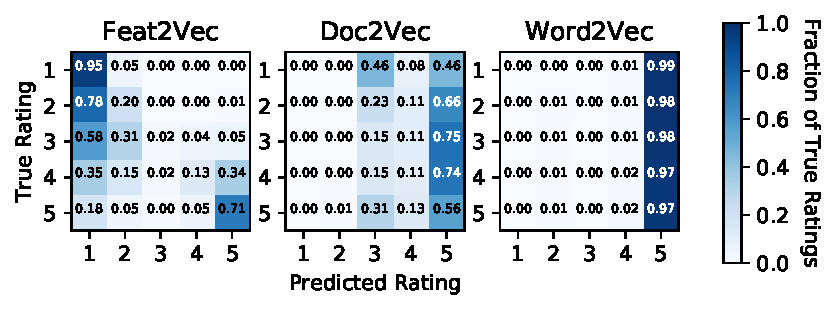
\includegraphics[width=.5\textwidth]{../paper/output/yelp/text_rating_confusionmat_numbers}
\caption{Confusion Matrices of Self-Supervised Yelp Ratings Predictions}
\label{fig:confmat}
\end{figure}
 %
 % \begin{table}
 % \centering
 % \caption{Self-Supervised Yelp rating prediction}
 % \label{ratingselfsup}
 % \begin{tabular}{lcc}
 % \toprule
 %                      & MSE   & Error Rate \\ \midrule
 % Random Rating     & 3.65 & 73\% \\
 % Feat2Vec             & 2.94 &  \textbf{55}\%       \\
 % Word2Vec            & 3.42 & 61\%                          \\
 % Doc2Vec              & \textbf{2.92}      & 73\% \\
 % \bottomrule
 % \end{tabular}
 % \end{table}

 \begin{comment}
We also vary $\alpha_1$, the flattening hyperparameter for feature group sampling, to see what effect this hyperparameter has on our performance. Intuitively, a low $\alpha_1$ will greatly improve the quality of the ratings embeddings learned, since it has relatively few parameters and is otherwise sampled infrequently. At the same time, with low $\alpha_1$ the director feature will be sampled less since it is one of the most complex features to learn, so the learned director embeddings may be of poorer quality. Figure \ref{fig:ratings} displays the results of our experiment, benchmarked against the performance of  $\Word2Vec$'s CBOW algorithm in the prediction task. We also show as a baseline the RMSE of a random uniform variable over the range of possible ratings (0 to 10). As is evident from the plot, CBOW performs a bit better than a random prediction, but is also handily outperformed by $\Feat2Vec$ across all hyper-parameter settings.
%There is no clear relation between $\alpha_1$ and the RMSE, suggesting
The algorithm's performance does not seem very sensitive to the hyperparameter choice.


%
% \begin{figure}
% \centering
% 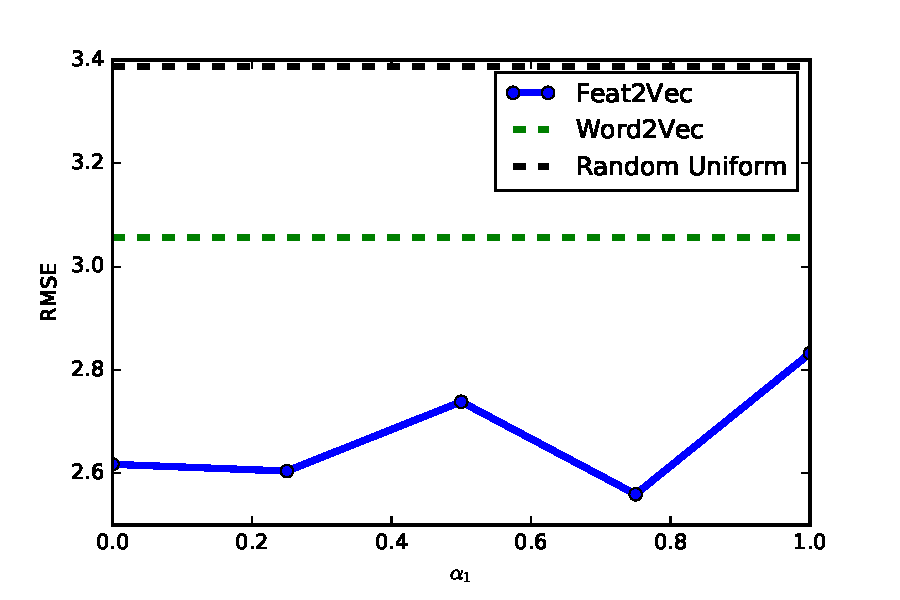
\includegraphics[scale=.4]{../paper/output/ratingsRankingRMSE.pdf}
% \caption{RMSE in Ratings Task as a Function of $\alpha_1$}
% \label{fig:ratings}
% \end{figure}
% \end{comment}


%\section{Relation to Prior Work}
%The original Factorization Machine formulation has been extended for multiple contexts.
%For example, Field-Aware Factrorization Machine~\cite{juan2016field} allows different weights for some feature interactions, but does not allow feature groups or feature extraction functions like Feat2Vec does.
%
%Algorithms that calculate continuous representations of entities other than words have been proposed for biological sequences~\cite{biovec}, of vertices in network graphs~\cite{Perozzi:2014:DOL:2623330.2623732}
%or in machine translation for embeddings of complete sentences~\cite{kiros2015skip}.
%Generative Adversarial Networks~\cite{goodfellow2014generative}(GANs) have been used to produce unsupervised embeddings of images effective for classification~\cite{radford2015unsupervised} and for generating natural language~\cite{press2017language}.
%To our knowledge, GANs have not been used for jointly embedding multiple feature types.
%Adversarial training could be an alternative to NCE for self-supervised learning, but we leave this for future study.


\section{Conclusion}
%Embeddings are useful tools in in Artificial Intelligence.
%Motivated by the success of $\Word2Vec$,

Embeddings have proven useful in a wide variety of contexts, but they are typically built from datasets with a single feature type as in the case of Word2Vec, or tuned for a single prediction task as in the case of Factorization Machine.
% In recent years, predictive tasks that traditionally have been solved with shallow models have been replaced with deep methods.
% However, as some critics point out, deep methods often work as black boxes, and  many times they are designed specifically for a single task with an arbitrary network that may not have much justification.
We believe $\Feat2Vec$ is an important step towards general-purpose methods, because
it decouples feature extraction from prediction for datasets with multiple feature types,  it can be self-supervised, and its embeddings are easily interpretable.


% We recently discovered a promising direction for an recent method called StarSpace~\cite{wu2017starspace} with similar goals from ours.
% %Even though they intend to be able to embed all types of features, at the time of the writing of this paper, their pre-print method was limited to only work for bag of words.
% %While $\Feat2Vec$ can jointly learn embeddings for all feature values in a dataset,  StarSpace samples a single arbitrary feature.
% StarSpace does not allow self-supervised learning and is not tested with features beyond bag of words
% %Our preliminary experiments suggest that sampling a single feature does not produce embeddings that generalize well.
% Nonetheless, a limitation of our work is that we do not compare with StarSpace, which future work may decide to do.


In the supervised setting,  $\Feat2Vec$ is able to calculate embeddings for passages of texts. We show  results  outperforming an algorithm specifically designed for text---even when using the same feature extraction CNN.
%This suggests that the need for  ad-hoc networks should be situated in relationship to the improvements over a general-purpose method.

%In the self-supervised setting, $\Feat2Vec$'s embeddings are able to capture relationships across features that can be twice as good as $\Word2Vec$'s CBOW algorithm on some evaluation metrics.
In the self-supervised setting, $\Feat2Vec$ exploits the structure of a dataset to learn embeddings in a more sensible way than existing methods. This yields performance improvements in our ranking and prediction tasks.
%The sampling method, and loss function that we use have interesting theoretical properties.
To the extent of our knowledge, Self-Supervised $\Feat2Vec$  is the first method to calculate continuous representations of data with multi-modal feature types and no explicit labels.



Future work could study how to reduce the amount of  human knowledge our approach requires;
for example by automatically grouping features into entities, or by automatically choosing a feature extraction function.
These ideas can extend to our codebase that we make available
\footnote{The code for the $\Feat2Vec$ algorithm is available \href{https://www.dropbox.com/sh/wdr2sgt0z9gj6kb/AABlzw7QhteTYViSoMk3CDZpa?dl=0}{here} and the experiments using the IMDB/Yelp data can be found
\href{https://www.dropbox.com/sh/uc07ng403i4ss9a/AAAPshFzdOug_ooeLn4SGR3Ua?dl=0}{here}.
}.
%Overall, we evaluate supervised and self-supervised Feat2Vec on 2 datasets each.
%Our evaluation is limited to two datasets---a public dataset that is freely available,  and a proprietary one that we are unable to distribute.
Though further experimentation is necessary, we believe that our results are an encouraging step towards general-purpose embedding models.


{
\footnotesize
\footnotesize
\bibliographystyle{aaai}
\bibliography{joseg}
}




\end{document}
